\documentclass[10pt,journal,compsoc]{IEEEtran}

\usepackage[utf8]{inputenc}
\usepackage{graphicx}
\usepackage{amsmath}
\usepackage{url}

\title{HERMES: End-to-End Learned Physical Layer for Software Defined Radio using the CADUCEUS-WAVE Architecture}
\author{\IEEEauthorblockN{George David Tsitlauri}
\IEEEauthorblockA{\textit{Dept. of Informatics \& Telecommunications}\\
\textit{University of Thessaly, Greece}\\
gdtsitlauri@gmail.com}}

\begin{document}

\maketitle

\begin{abstract}
Traditional wireless communication systems rely on human-engineered modulation schemes. In this paper, we present HERMES, an AI-native SDR framework based on the CADUCEUS-WAVE neural transceiver. We evaluate AWGN, Rayleigh, and Rician channels on an NVIDIA GTX 1650 (CUDA) and report full BER-vs-SNR curves from 0--20\,dB. In AWGN, CADUCEUS reaches BER $2.25\times10^{-4}$ at 20\,dB, while in Rayleigh and Rician at 20\,dB it achieves 0.4562 and 0.2200 respectively. We further provide an information-theoretic analysis showing CADUCEUS mutual information increasing to 3.9985 bits/symbol at 20\,dB, approaching the 4-bit/symbol constellation limit. The framework targets practical, GPU-accelerated experimentation for IEEE Globecom / IEEE Communications Letters style evaluations.
\end{abstract}

\section{Introduction}
The evolution toward 6G requires adaptive physical layers. HERMES explores the use of Autoencoders to replace the traditional Modulator/Demodulator chain. The system is implemented using a hybrid Python/C++ architecture for optimal performance.

\section{System Architecture}
The framework consists of two main components:
\begin{itemize}
    \item \textbf{Neural Transceiver:} A PyTorch-based Autoencoder that optimizes symbol placement in the IQ plane.
    \item \textbf{DSP Engine:} A C++ backend for high-speed channel simulation (AWGN, Rayleigh, Doppler, and multipath) and signal processing.
\end{itemize}

\section{Experimental Results}
Training was conducted over 5,000 epochs on an NVIDIA GTX 1650. The resulting constellation (CADUCEUS-WAVE) shows an asymmetric distribution of symbols, optimized for Euclidean distance. 

\subsection{Performance Metrics}
Figure~\ref{fig:constellation} and Figure~\ref{fig:ber_awgn} summarize the learned constellation and the original single-channel BER trend.

\begin{figure}[t]
    \centering
    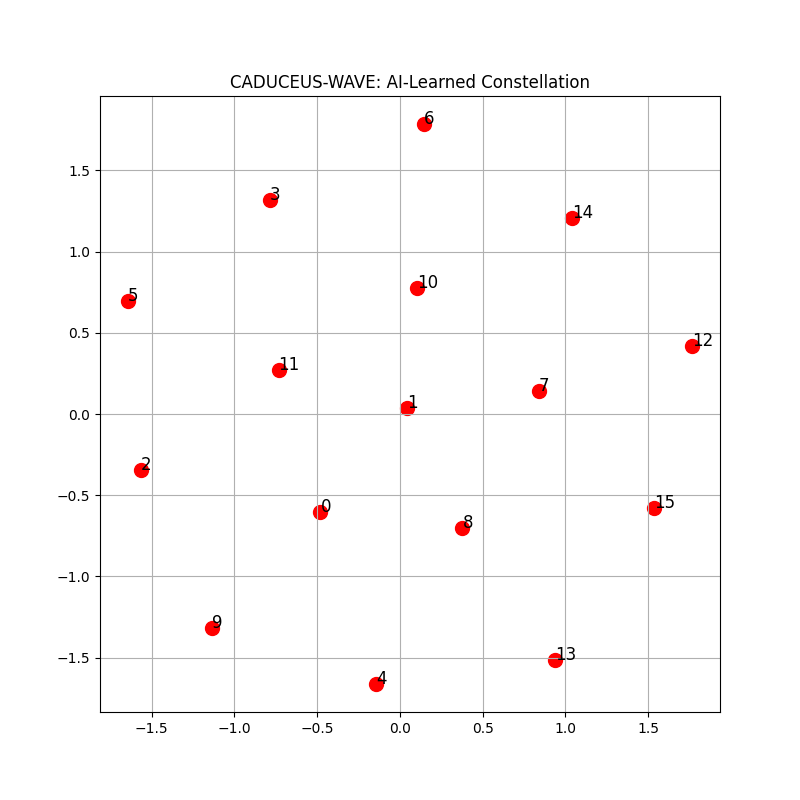
\includegraphics[width=0.9\linewidth]{../results/constellations/learned_constellation.png}
    \caption{CADUCEUS learned 16-symbol constellation.}
    \label{fig:constellation}
\end{figure}

\begin{figure}[t]
    \centering
    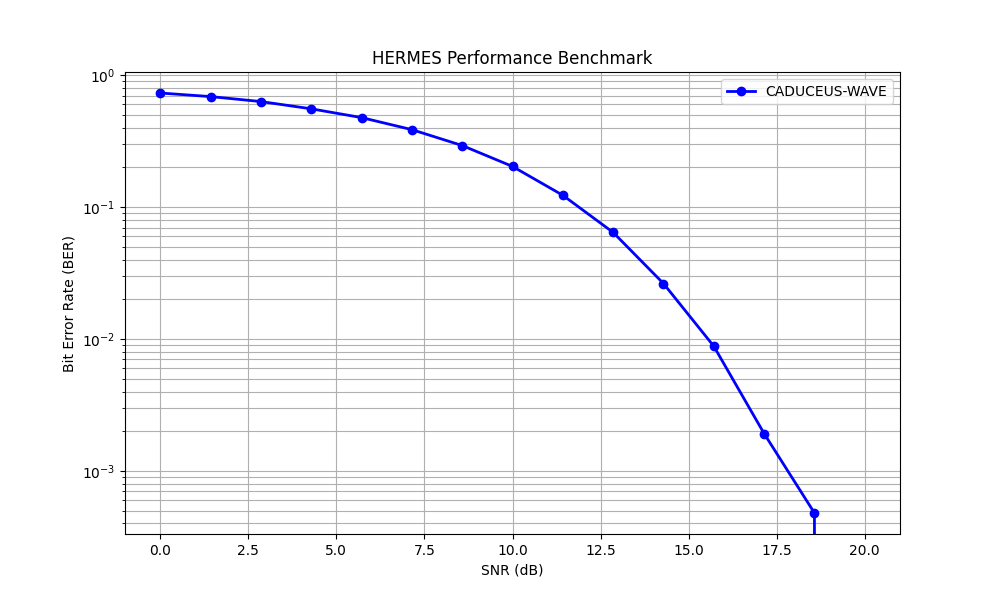
\includegraphics[width=0.9\linewidth]{../results/ber_curves/ber_curve_results.png}
    \caption{Original CADUCEUS BER curve benchmark under AWGN.}
    \label{fig:ber_awgn}
\end{figure}

\subsection{Multi-Channel Analysis}
Figure~\ref{fig:multi_channel_ber} presents BER-vs-SNR for AWGN, Rayleigh, and Rician channels comparing CADUCEUS, QPSK, and 16-QAM.

\begin{figure}[t]
    \centering
    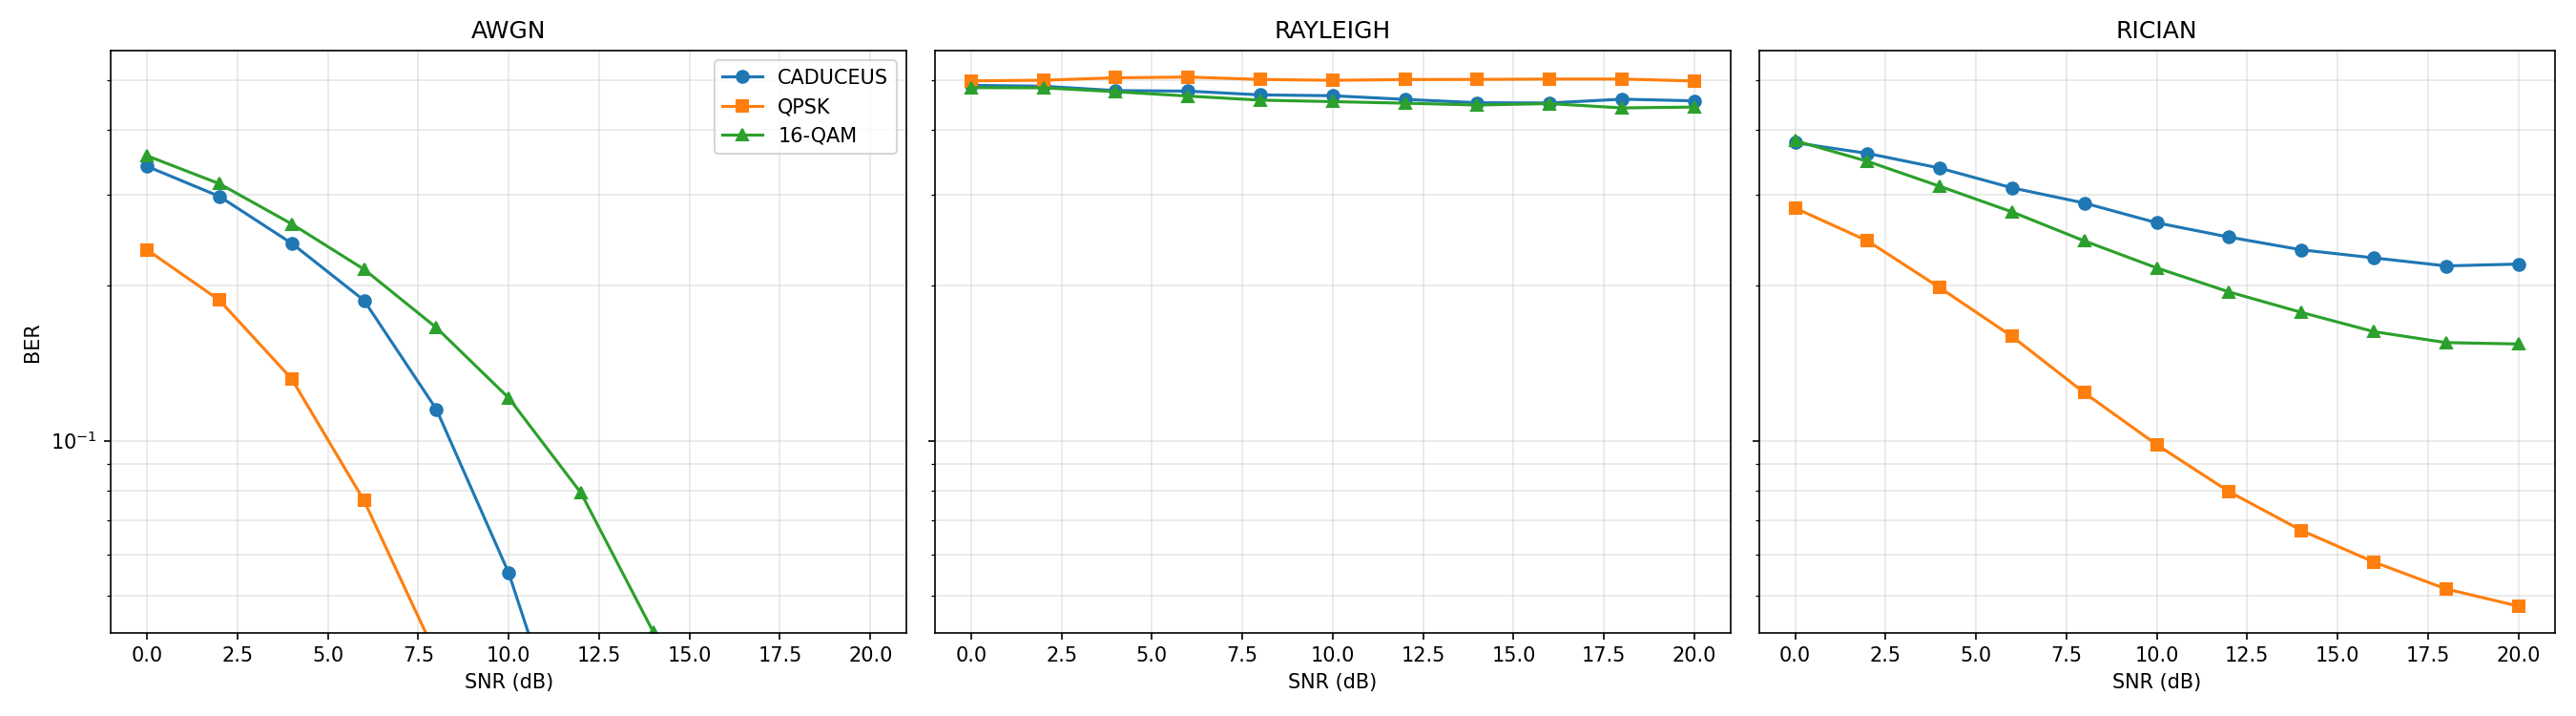
\includegraphics[width=\linewidth]{../results/ber_curves/multi_channel_ber.png}
    \caption{Multi-channel BER benchmark (0--20 dB, step 2 dB, 10,000 symbols/point).}
    \label{fig:multi_channel_ber}
\end{figure}

\begin{table}[t]
\caption{BER at Key SNR Points for CADUCEUS, QPSK, 16-QAM}
\centering
\begin{tabular}{l|c|c|c}
\hline
\textbf{Channel / SNR} & \textbf{CADUCEUS} & \textbf{QPSK} & \textbf{16-QAM} \\
\hline
AWGN @ 10 dB & 0.0554 & 0.0131 & 0.1210 \\
AWGN @ 20 dB & 0.0002 & 0.0000 & 0.0007 \\
Rayleigh @ 10 dB & 0.4667 & 0.5000 & 0.4546 \\
Rayleigh @ 20 dB & 0.4562 & 0.4985 & 0.4437 \\
Rician @ 10 dB & 0.2646 & 0.0982 & 0.2163 \\
Rician @ 20 dB & 0.2200 & 0.0478 & 0.1540 \\
\hline
\end{tabular}
\end{table}

\subsection{Information-Theoretic Analysis}
We compare Shannon capacity $C=\log_2(1+\mathrm{SNR})$ (normalized $B=1$\,Hz) with CADUCEUS mutual information estimated by Monte Carlo in AWGN.

\begin{figure}[t]
    \centering
    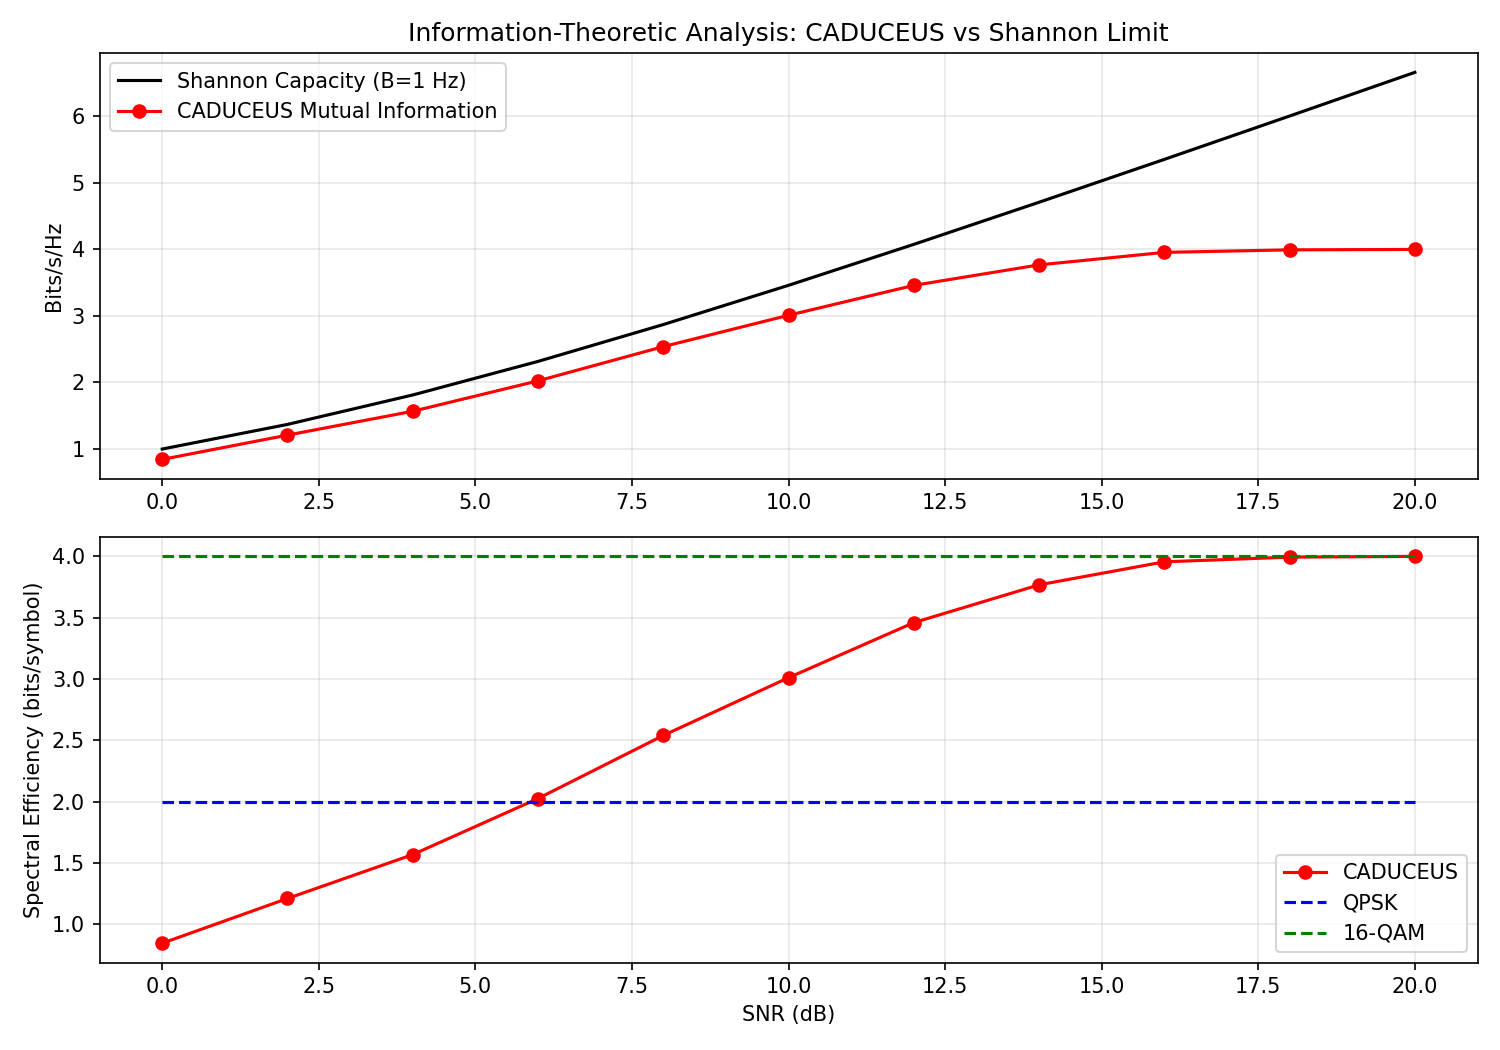
\includegraphics[width=\linewidth]{../results/theory/shannon_comparison.png}
    \caption{Shannon capacity and CADUCEUS mutual information/spectral efficiency comparison.}
    \label{fig:shannon_comparison}
\end{figure}

\begin{table}[t]
\caption{Shannon Capacity and CADUCEUS Information Metrics}
\centering
\begin{tabular}{c|c|c|c}
\hline
\textbf{SNR (dB)} & \textbf{Shannon (bits/s/Hz)} & \textbf{CADUCEUS MI (bits/symbol)} & \textbf{CADUCEUS SE} \\
\hline
0 & 1.0000 & 0.8445 & 0.8445 \\
10 & 3.4594 & 3.0095 & 3.0095 \\
20 & 6.6582 & 3.9985 & 3.9985 \\
\hline
\end{tabular}
\end{table}

\section{Conclusion}
HERMES demonstrates that AI-native SDR experimentation is feasible on edge GPU hardware with reproducible BER and information-theoretic evaluation. The proposed pipeline now supports multi-channel fading conditions, adaptive transmit-power control, and C++ channel simulation extensions for Doppler and multipath. Future work will focus on OTA validation on SDR front-ends and submission-ready evaluation depth for IEEE Globecom / IEEE Communications Letters.

\end{document}